\begin{figure*}[htbp]
    \centering
    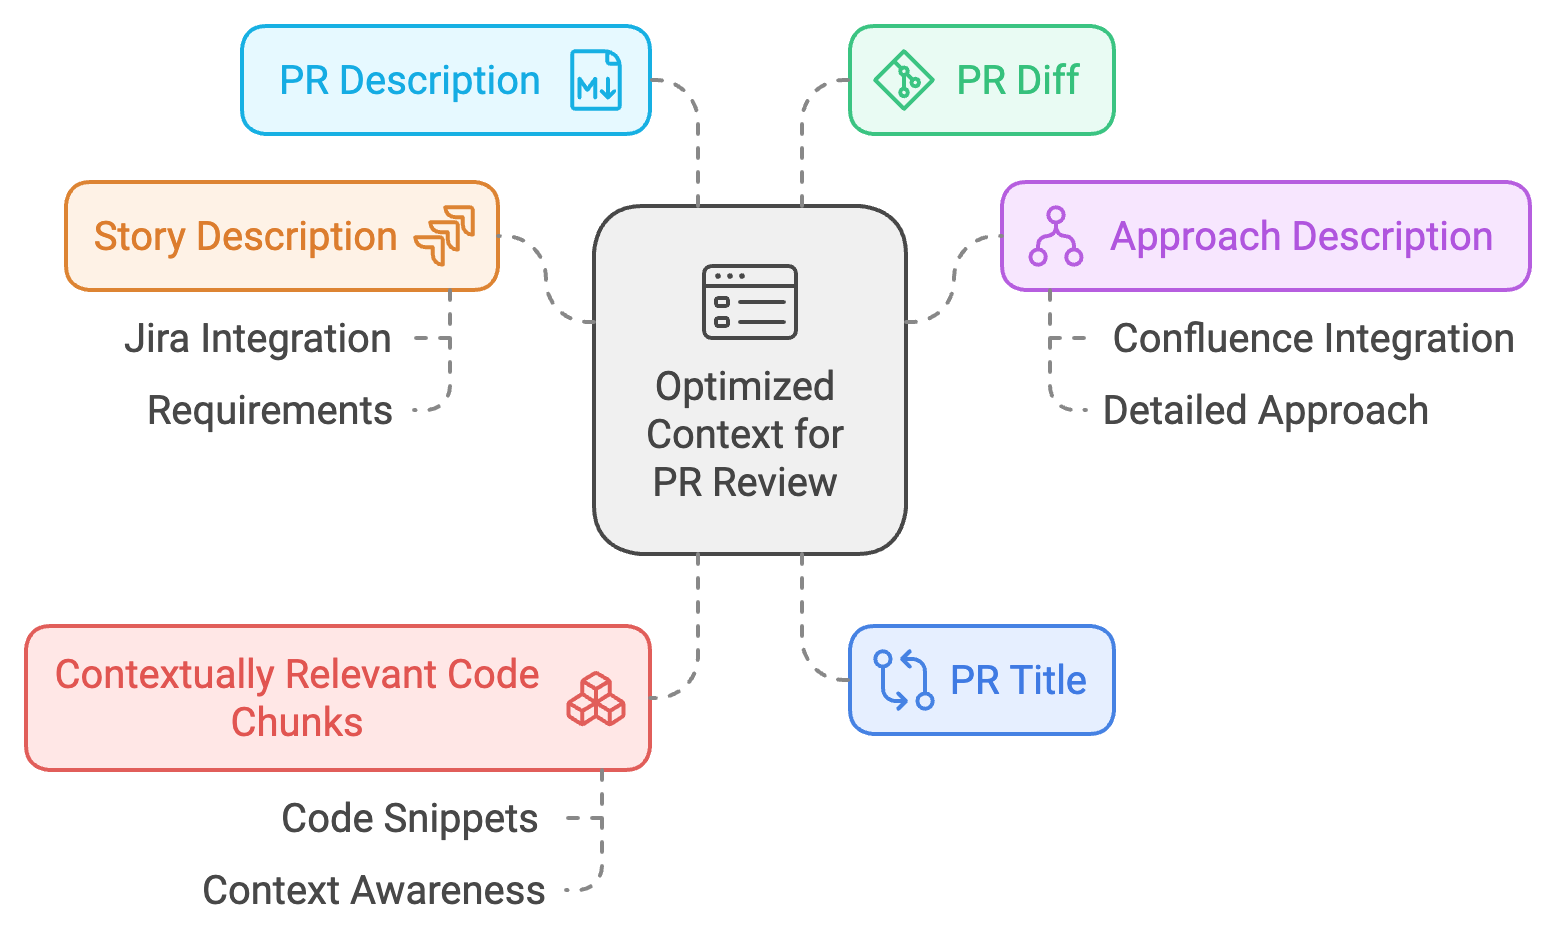
\includegraphics[width=0.8\textwidth]
    {Figures/context_creation.png}
    \caption{DeputyDev fetches relevant information from multiple sources and unionize them smartly to create an optimized context. This context is self sufficient to provide all necessary information while reviewing PR.}
    \label{fig:context-creation}
\end{figure*}

\section{Approach}
Collating all pieces of context requires extensive integration with sources. For PR title, description and diff, DeputyDev can integrate with popular version control systems like Github, Gitlab and Bitbucket.

For story and approach description DeputyDev integrates with Atlassian suite i.e Jira and Confluence. Every PR being raised should have an associated Jira story or confluence page (mentioned in description of PR). DeputyDev will then pull their contents and format them to be included in optimized context.

Lastly, the most crucial piece of information that makes DeputyDev powerful and context-aware is contextually relevant code chunks. These relevant code chunks are fetched and stored ephemerally while the review process is ongoing. Let us understand with an example what exactly is a contextually relevant code chunk.\ref{fig:context-creation}


Original code
\begin{lstlisting}
def calculate_total(items):
    return sum(item.price for item in items)

def apply_discount(total, discount_percent):
    return total * (1 - discount_percent / 100)

def process_order(items, discount_percent=0):
    total = calculate_total(items)
    final_price = apply_discount(total, discount_percent)
    return final_price

# Example of where process_order is called
class OrderService:
    def create_order(self, user_id, items):
        user = get_user(user_id)
        discount = user.loyalty_discount
        total = process_order(items, discount)
        return Order(user=user, items=items, total=total)
\end{lstlisting}

Diff (Changes to be Made)

\begin{lstlisting}[escapechar=|]
def process_order(items, discount_percent=0):
    total = calculate_total(items)
    if discount_percent > 50:
        raise ValueError("Discount cannot exceed 50%")
    final_price = apply_discount(total, discount_percent)
    return final_price
\end{lstlisting}

Consider a simple code example above and let's break down the contextually relevant code chunks:

\begin{enumerate}
    \item \texttt{calculate\_total} and \texttt{apply\_discount} functions: As mentioned before, these are called within \texttt{process\_order} and remain relevant.
    \item \texttt{OrderService.create\_order} method: This is now a crucial contextually relevant code chunk. It calls \texttt{process\_order} and would be affected by the PR changes in the following ways:
    \begin{itemize}
        \item It might now raise a ValueError if a user's loyalty discount exceeds 50\%.
        \item The error handling in this method (not shown) might need to be updated to catch and handle the new potential ValueError.
    \end{itemize}
    \item \texttt{User} model or class: Although not fully shown, the existence of \texttt{user.loyalty\_discount} suggests there's a User model or class. This becomes contextually relevant because:
    \begin{itemize}
        \item We need to ensure that loyalty discounts in the system never exceed 50\%, or handle cases where they might.
        \item There might be a need to update the User model or associated business logic to cap loyalty discounts at 50\%.
    \end{itemize}
    \item \texttt{Order} model or class: The \texttt{Order} being created with the total from \texttt{process\_order} is relevant because:
    \begin{itemize}
        \item It assumes \texttt{process\_order} always returns a valid total.
        \item If \texttt{process\_order} now throws an exception, we need to ensure the Order creation process can handle this.
    \end{itemize}
\end{enumerate}

This example illustrates how a seemingly small change to \texttt{process\_order} has ripple effects throughout the system. When reviewing the PR, a developer would need to consider:

\begin{itemize}
    \item How to handle potential ValueErrors in the \texttt{OrderService} and potentially other services.
    \item Whether the \texttt{User} model and associated business logic need updates to prevent invalid discount values.
    \item If there are other parts of the system that rely on discounts never being rejected, which might now break.
\end{itemize}

By identifying these contextually relevant code chunks, DeputyDev can perform a more comprehensive review, anticipating potential issues and ensuring that the PR's changes integrate smoothly with the entire system.

A counterpoint to our method of selecting relevant code snippets might be: "Why not just input the entire codebase?" However, this approach faces several challenges:

\begin{enumerate}
    \item \textbf{Limited context window of LLMs}: Though most capable LLMs now support more than 100k context window, It can still prove to be insufficient for large codebases
    \item \textbf{Lost in the middle problem}: The "lost in the middle" problem occurs when LLMs process long texts. They tend to focus on the beginning and end, while losing track of important information in the middle. This is similar to how humans might remember the start and conclusion of a long lecture, but struggle to recall specific details from the middle portion.
    \item \textbf{Cost considerations}: Sending an entire codebase to LLMs as context can be costly.
\end{enumerate}

\begin{figure*}[htbp]
    \centering
    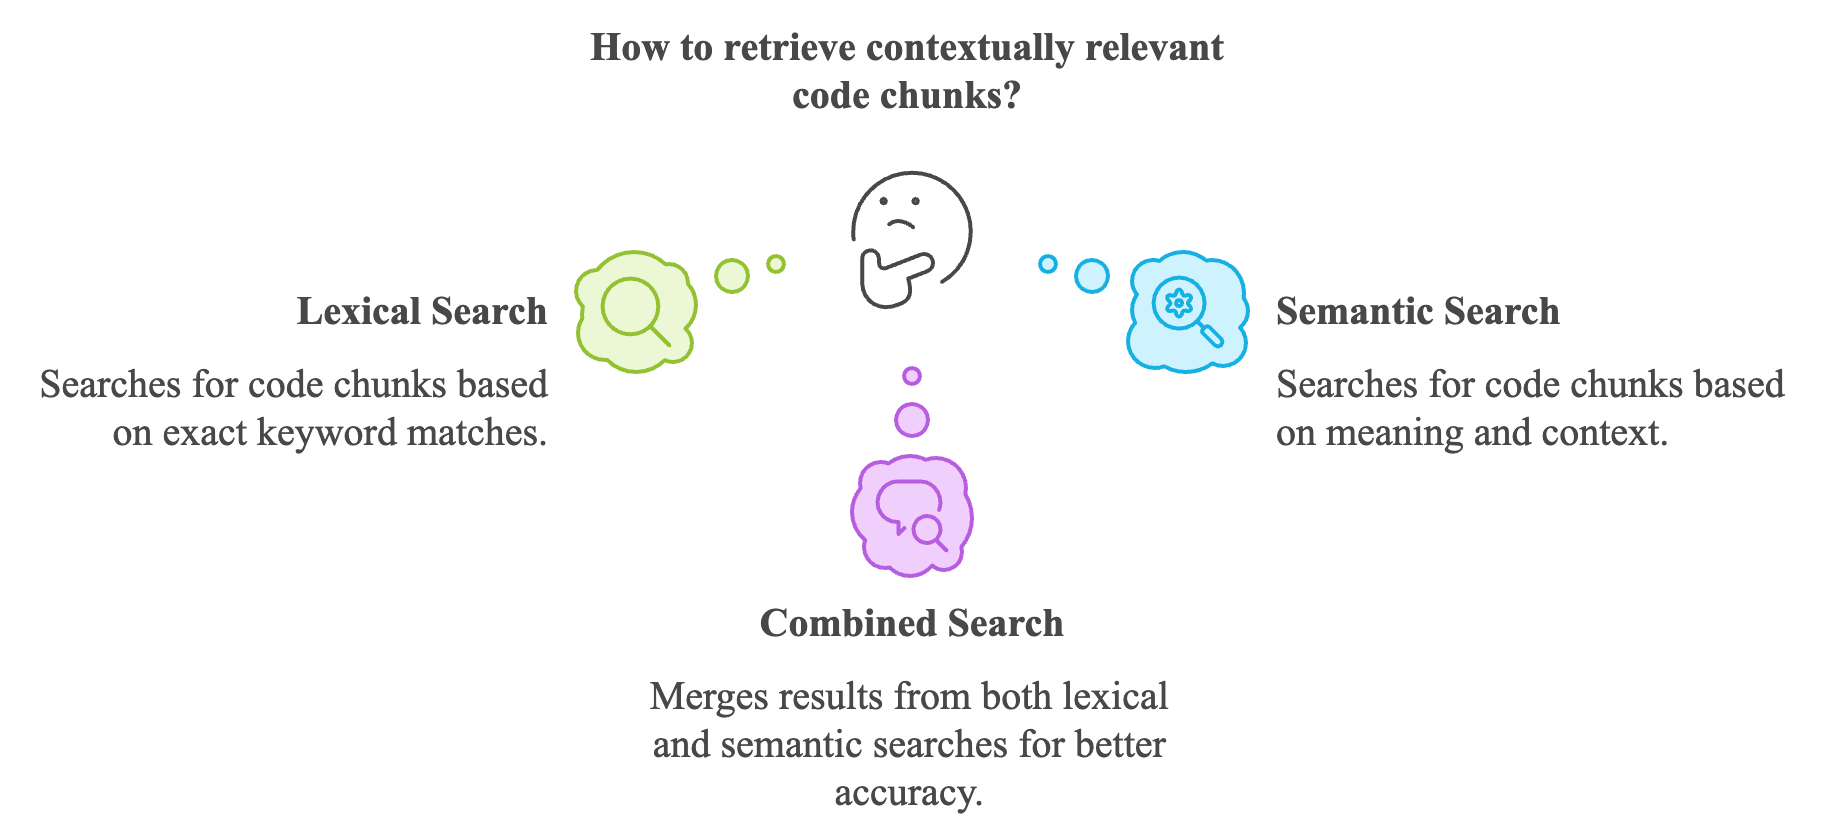
\includegraphics[width=0.8\textwidth]
    {Figures/search.png}
    \caption{Obtaining contextually relevant code chunks is crucial for code review to happen effectively. This process involves lexical and semantic search and then combining both their results together.
}
    \label{fig:DeputyDev-search}
\end{figure*}